\chapter{第一次使用：先看懂工作台}

\section{先看一次完整任务，再学习背后的阶段}

这章的目的不是让你先背一堆 Agent 术语，而是先知道“使用者到底在页面上做什么”。我们先完成一个完整任务：\textbf{比较两个候选商品的噪声反馈}。之后再把页面上的每一步，接回 P0--P7 的开发过程。

\begin{boundarybox}
本章截图来自 synthetic 工作台（合成演示数据）。它不调用 DeepSeek，也不读取真实评论；它只能帮助你看懂页面和任务流，不能证明真实业务效果、节省工时或真人愿意使用。
\end{boundarybox}

\begin{beginnerbox}
先记住一句话：左边决定“做哪种运营任务”，中间告诉系统“看哪些商品、哪个问题”，右边告诉你“系统现在得到什么、下一步做什么”。你可以把它看成一张任务单，而不是一个可以随便聊天的机器人。
\end{beginnerbox}

\section{第一次打开：页面在问你要解决什么问题}

打开电脑浏览器中的本地工作台后，默认会看到一个单品体验诊断页面。此时还没有运行结果，页面是在等待你填写任务条件。

\begin{figure}[htbp]
  \centering
  \IfFileExists{assets/p7-tour-01-initial.png}{%
    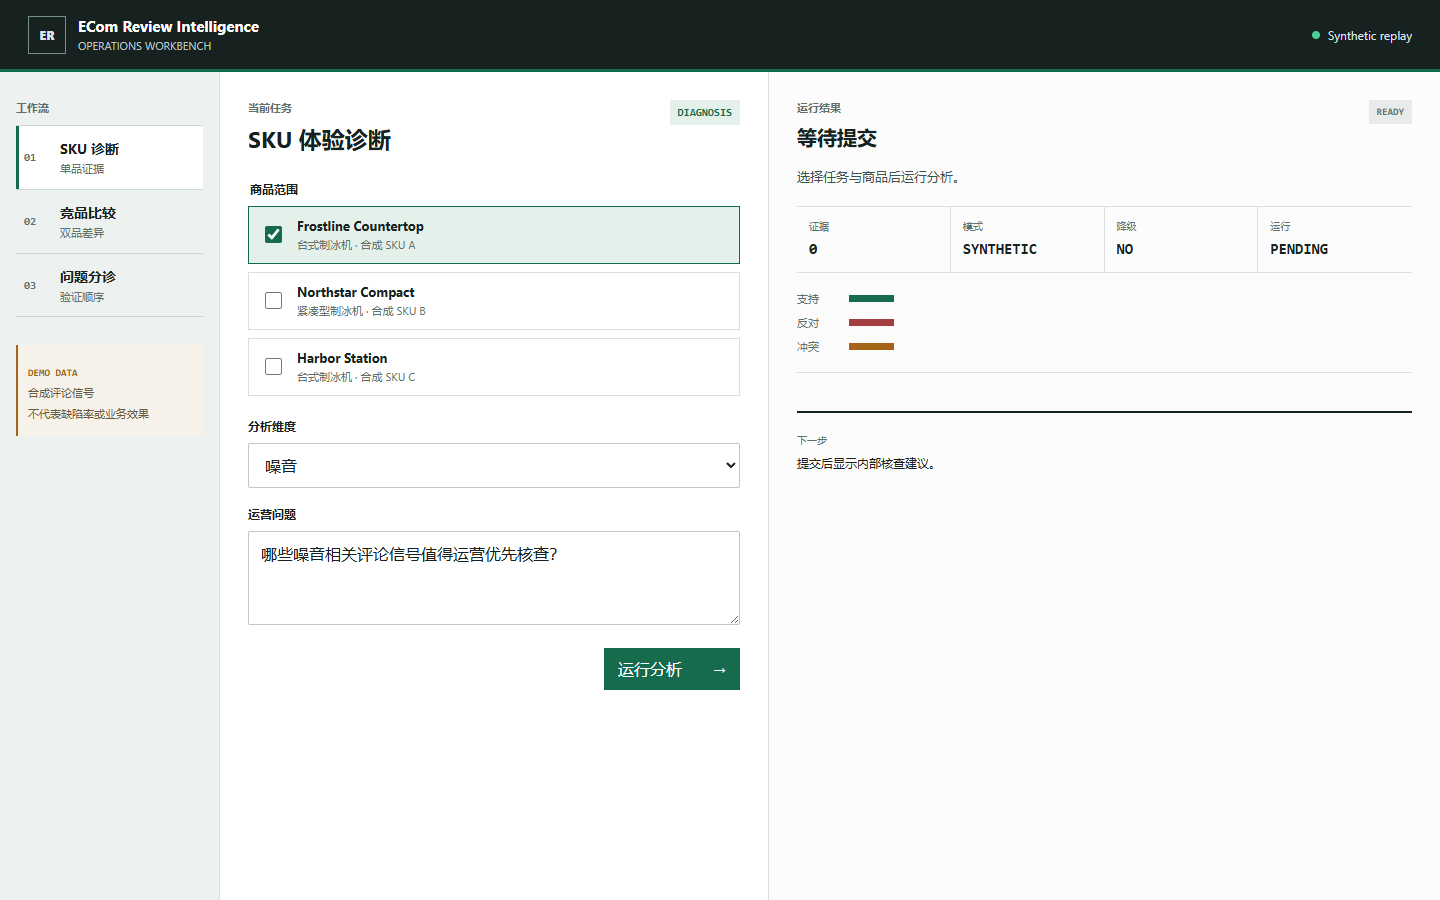
\includegraphics[width=\textwidth]{assets/p7-tour-01-initial.png}%
  }{%
    \fbox{\parbox[c][45mm][c]{0.90\textwidth}{\centering
      此处放置电脑端截图\\
      \texttt{assets/p7-tour-01-initial.png}\\
      synthetic 初始页面}}
  }
  \caption{第一次打开 synthetic 工作台：尚未提交任务。}
\end{figure}

这张图先看五个位置。\textbf{左侧工作流导航}列出单品诊断、竞品比较和问题分诊；\textbf{中间商品与问题选择}让使用者选择商品、分析维度和运营问题；页面下方的\textbf{运行按钮}负责提交这张任务单；\textbf{右侧状态}此时显示等待提交，还没有证据；右侧底部的\textbf{下一步}告诉你提交后会出现结果。\textbf{这一屏在项目中要展现什么：}使用者先从一个明确任务开始，而不是把目标交给模型自由猜。

初学者不需要一次读懂所有英文。先按“左边选任务 $→$ 中间填条件 $→$ 点击运行 $→$ 右边读结果”的方向扫一遍，再回头看细节。页面上的英文状态只是程序用来传递状态的固定标签，中文说明才是这次演示应该采取的动作。

\begin{longtable}{>{\raggedright\arraybackslash}p{0.18\textwidth}>{\raggedright\arraybackslash}p{0.31\textwidth}>{\raggedright\arraybackslash}p{0.35\textwidth}}
\toprule
位置 & 截图里看到的内容 & 先问自己的问题 \\
\midrule
\endfirsthead
\toprule
位置 & 截图里看到的内容 & 先问自己的问题 \\
\midrule
\endhead
左侧导航 & 三种任务：单品诊断、商品比较、问题分诊。 & 我现在要回答的是“看一个商品”“比较商品”，还是“决定先查哪件事”？ \\
中间表单 & 商品、分析维度、运营问题。 & 系统究竟要看谁、看哪个问题、回答什么？ \\
运行按钮 & 提交一次受控任务。 & 条件填好了吗？点击后是否会产生一次可追踪运行？ \\
右侧状态 & 等待、已验证或需要澄清。 & 结果能不能直接使用，还是要先补信息？ \\
右侧证据与下一步 & 聚合信号、证据卡和建议动作。 & 结论依据是什么？运营人员下一步要核查什么？ \\
\bottomrule
\end{longtable}

\begin{beginnerbox}
这一页的业务价值是把“我感觉这个商品可能有问题”改写成一张可以复核的任务单。任务单越明确，后面越容易知道结果回答了什么，也越容易把结果交给客服、品类或质量团队继续处理。
\end{beginnerbox}

\section{先完成一次单品诊断：看一个商品的噪声反馈}

第一次可以先保留默认的“单品诊断”（diagnosis），选择一个商品，把分析维度选为“噪音”，并将问题写成“哪些噪音相关评论信号值得运营优先核查？”。这里的商品名称只是 synthetic 页面中的演示名称，不是公开手册中的真实商品标识。

\begin{figure}[htbp]
  \centering
  \IfFileExists{assets/p7-tour-02-diagnosis.png}{%
    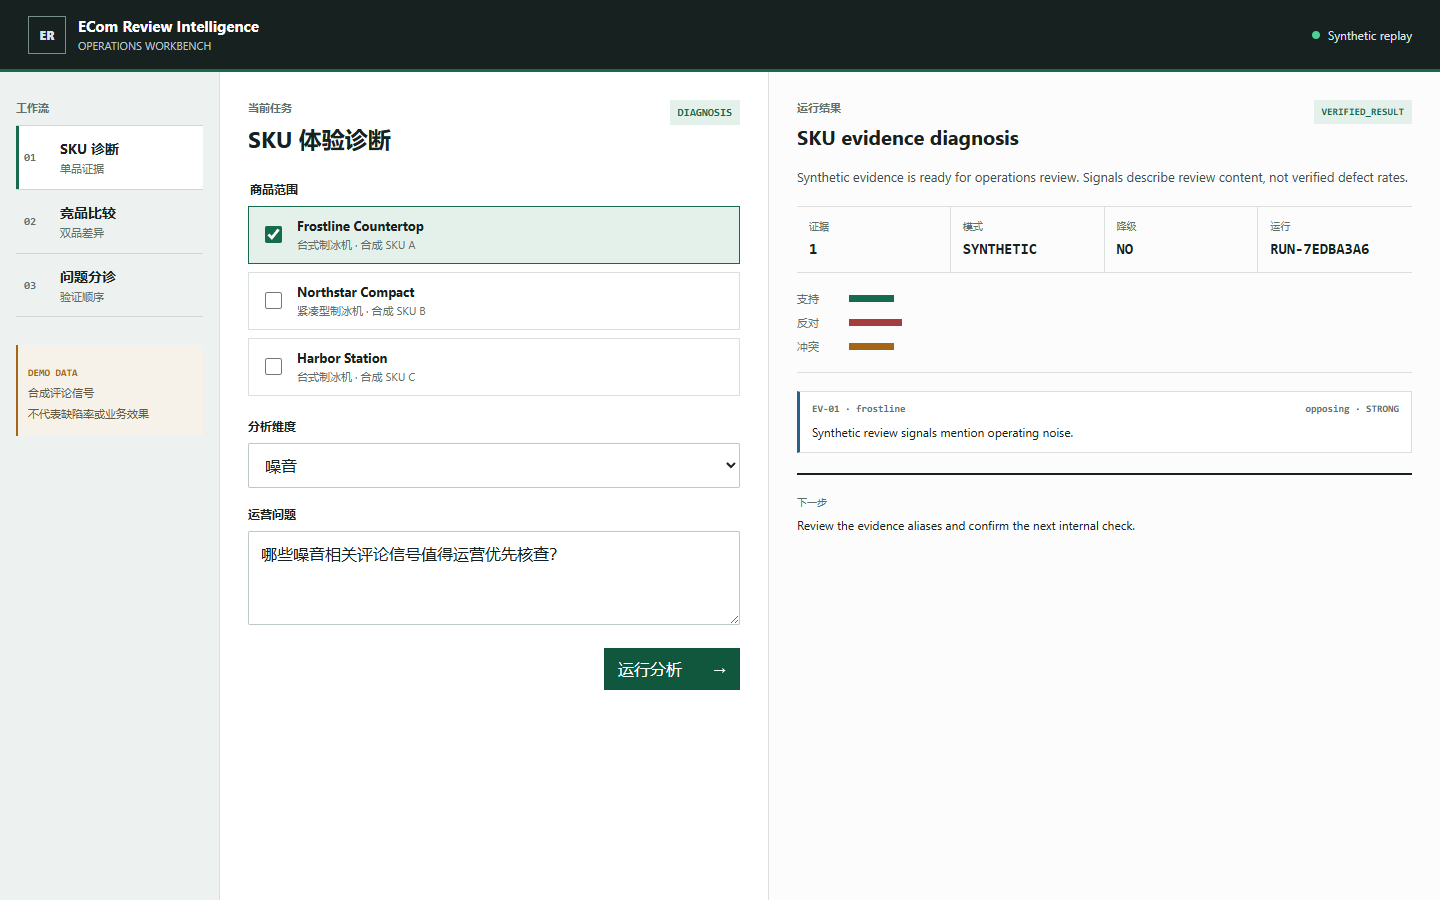
\includegraphics[width=\textwidth]{assets/p7-tour-02-diagnosis.png}%
  }{%
    \fbox{\parbox[c][45mm][c]{0.90\textwidth}{\centering
      此处放置电脑端截图\\
      \texttt{assets/p7-tour-02-diagnosis.png}\\
      单品诊断结果}}
  }
  \caption{运行单品诊断后，查看状态、证据和下一步。}
\end{figure}

这一屏中，\textbf{左侧工作流导航}高亮单品诊断；\textbf{中间区域}保留一个商品、一个分析维度和一个运营问题；\textbf{运行按钮}是任务提交的唯一入口；\textbf{右侧状态}告诉你结果是否完成检查；\textbf{右侧证据}展示匿名的聚合信号和证据卡；\textbf{右侧下一步}提示运营人员继续核查。\textbf{这一屏在项目中要展现什么：}先把“一个商品的一个问题”跑通，再理解系统如何给出可复核的证据提示。

\subsection*{结果页怎么读：先状态，后范围，再证据}

建议固定使用下面的顺序，不要先被右侧的一句英文总结带着走：

\begin{enumerate}
  \item \textbf{先看状态。}截图中的 \texttt{VERIFIED\_RESULT} 表示这次合成运行通过了本地规则检查；它表示“这份结果在当前演示边界内可继续查看”，不表示商品缺陷已经被现实世界证实。
  \item \textbf{再看范围和数量。}\texttt{SYNTHETIC} 表示数据是合成演示数据，数量表示本次允许使用的商品或证据规模；它们帮助你判断结果覆盖多大范围。
  \item \textbf{再看彩色信号条。}绿色、红色和橙色分别代表支持、反对和冲突方向。条形长短只用于比较当前演示中的相对信号，不是百分比、评分或缺陷率。
  \item \textbf{再看证据卡。}证据卡把某个信号和商品别名连起来，方便人回到本地证据账本核查；卡片中的匿名编号是本地演示 ID，不是官方 Amazon review ID。
  \item \textbf{最后看下一步。}下一步是运营动作提示，例如复核证据或确认内部检查，不是模型替人下达的采购、下架或赔付决定。
\end{enumerate}

\begin{longtable}{>{\raggedright\arraybackslash}p{0.22\textwidth}>{\raggedright\arraybackslash}p{0.34\textwidth}>{\raggedright\arraybackslash}p{0.28\textwidth}}
\toprule
右侧栏位 & 它在本项目里的功能 & 不能从它推出什么 \\
\midrule
\endfirsthead
\toprule
右侧栏位 & 它在本项目里的功能 & 不能从它推出什么 \\
\midrule
\endhead
状态 & 告诉使用者流程是否完成检查。 & 不能推出真实质量结论。 \\
范围与数量 & 说明本次运行使用的演示范围。 & 不能推出全市场样本量。 \\
信号条 & 让不同方向的聚合信号一眼可比。 & 不能当作概率、占比或 ROI。 \\
证据卡 & 给出可回查的本地证据线索。 & 不能当作原始评论全文或官方评论 ID。 \\
下一步 & 把结果交给合适的人工核查动作。 & 不能当作自动执行外部业务操作。 \\
\bottomrule
\end{longtable}

\begin{beginnerbox}
看完这张诊断图，初学者只要能回答三句话就算读懂了：\textbf{系统看的是哪个商品？它观察到的信号方向是什么？我下一步要回查哪条证据？}如果答不出来，先不要急着学习模型名称。
\end{beginnerbox}

\section{这一次运行得出了什么：把结果读成分析结论}

前面两节教的是“怎么点、按什么顺序看”。这一节回答更进一步的问题：右侧得出的这份结果，\textbf{代表了什么样的分析结论？拿到它能做什么业务动作？在项目当前阶段，它又意味着什么？}

\subsection{先分清：合成模式的数字是“演示值”，不是“计算值”}

\begin{factbox}
诊断截图中的 \texttt{EV-01}、\texttt{opposing}、\texttt{STRONG} 和三条信号条，全部来自确定性代码按固定规则生成的合成数据：单品诊断固定返回一张反对方向、STRONG 强度的证据卡。它们不来自任何真实评论的计算，因此这些数值本身没有业务含义；有学习意义的是结果的\textbf{结构}——状态、范围、方向、强度和下一步如何组合成一份可复核的结论。
\end{factbox}

这也解释了一个容易困惑的点：截图里只有一张证据卡，强度却标着 \texttt{STRONG}。在真实证据体系里，STRONG 表示“五条及以上匹配记录”；在合成模式里，它只是固定的演示标签。把“标签的定义”和“标签的来源”分开，是读懂任何模式的第一步。

\subsection{把任意一次结果读成一句结论}

无论合成、受控本地还是真实模式，都可以套用同一个结论模板：

\begin{beginnerbox}
“在〈模式标注的范围〉内，〈商品〉在〈维度〉上，系统给出〈强度〉的〈方向〉信号，下一步应〈下一步内容〉。”

套用到诊断截图即：“在合成演示范围内，Frostline 在噪音维度上给出一条 STRONG 的反对方向信号，下一步是复核证据编号并确认内部检查。”这句话就是本次运行“代表的分析结论”。注意它自带范围限定语；把限定语去掉（例如说成“Frostline 噪音有问题”），就越过了证据边界。
\end{beginnerbox}

结果页右侧各字段与结论、业务动作的对应关系如下：

\begin{longtable}{>{\raggedright\arraybackslash}p{0.18\textwidth}>{\raggedright\arraybackslash}p{0.24\textwidth}>{\raggedright\arraybackslash}p{0.24\textwidth}>{\raggedright\arraybackslash}p{0.18\textwidth}}
\toprule
字段（截图值） & 它代表的分析结论 & 拿到后可做的业务动作 & 它不能推出什么 \\
\midrule
\endfirsthead
\toprule
字段（截图值） & 它代表的分析结论 & 拿到后可做的业务动作 & 它不能推出什么 \\
\midrule
\endhead
\texttt{VERIFIED\_RESULT} & 本地检查通过、引用一致 & 继续逐卡阅读证据 & 商品质量合格 \\
模式 \texttt{SYNTHETIC} & 数字是固定演示值 & 练习读法、演示流程 & 任何真实统计 \\
证据 1 & 本次产出一卡 & 按编号回查 & 评论总数或样本量 \\
方向 \texttt{opposing} & 该卡为反对方向 & 复核客诉、补充详情页说明、列入质检关注 & 差评率 \\
强度 \texttt{STRONG} & 真实体系=五条以上匹配；合成=演示标签 & 安排核查优先级 & 问题严重度 \\
冲突信号条 & 同维度支持与反对并存（两极分化） & 人工回到原始证据下结论 & 好评差评占比 \\
下一步 & 人工核查建议 & 安排内部复核或派单 & 自动执行的动作 \\
\bottomrule
\end{longtable}

\subsection{页面英文词速查}

\begin{longtable}{>{\raggedright\arraybackslash}p{0.34\textwidth}>{\raggedright\arraybackslash}p{0.58\textwidth}}
\toprule
页面英文 & 中文含义 \\
\midrule
\endfirsthead
\toprule
页面英文 & 中文含义 \\
\midrule
\endhead
\texttt{READY} / \texttt{PENDING} & 待提交 / 等待运行 \\
\texttt{VERIFIED\_RESULT} & 已验证结果：本地校验通过，可以往下看 \\
\texttt{CLARIFICATION\_REQUIRED} & 需要澄清：商品不唯一，等人选择后继续 \\
\texttt{DEGRADED\_SAFE\_RESULT} & 安全降级：复核失败后返回的保守失败结果 \\
\texttt{SYNTHETIC} / \texttt{LOCAL} & 合成演示数据 / 受控本地真实数据 \\
\texttt{supporting} / \texttt{opposing} / \texttt{conflicting} & 支持 / 反对 / 冲突（同一维度两极分化） \\
\texttt{STRONG} / \texttt{MODERATE} / \texttt{WEAK} / \texttt{INSUFFICIENT} & 强（5 条及以上）/ 中（2--4 条）/ 弱（1 条）/ 证据不足（0 条） \\
\texttt{degraded: YES / NO} & 本次运行是否发生过安全降级 \\
\bottomrule
\end{longtable}

\subsection{三个工作流分别支撑什么业务动作}

\begin{longtable}{>{\raggedright\arraybackslash}p{0.18\textwidth}>{\raggedright\arraybackslash}p{0.40\textwidth}>{\raggedright\arraybackslash}p{0.32\textwidth}}
\toprule
工作流 & 结果支撑的业务动作 & 系统不替你做的事 \\
\midrule
\endfirsthead
\toprule
工作流 & 结果支撑的业务动作 & 系统不替你做的事 \\
\midrule
\endhead
单品诊断 & 判断是否优先复核该商品的客诉、是否在详情页补充说明、是否把该维度列入质检关注 & 不决定下架、召回或赔付 \\
竞品比较 & 为选品评审提供同一维度下的证据对比输入 & 不宣布哪个商品更好，不给采购结论 \\
问题分诊 & 决定先派给质量、客服等哪个团队，排出核查顺序 & 不自动派单，不估算业务损失 \\
\bottomrule
\end{longtable}

\begin{advicebox}
动作模板本身是真实的运营用法；但在合成阶段，证据内容是演示值，这些动作此刻只能“演练”。真实动作需要受控本地或真实模式提供可回查的证据，并经目标运营用户试用验证。
\end{advicebox}

\subsection{当前阶段，这份结果意味着什么}

\begin{factbox}
现阶段（synthetic）这份结果证明的工程事实是：任务单提交、状态标记、证据卡渲染和下一步提示的完整链路按设计工作。它是界面与流程的工程演示证据。
\end{factbox}

\begin{boundarybox}
它不证明系统对真实商品的分析正确，也不证明能节省工时或改善决策。当前项目状态为 P7 进行中：目标运营用户的结构化试用尚未完成，业务效果仍属待验证。把三种模式连起来看会更清楚：合成模式证明“页面与流程会正确地动”；受控本地模式让数字来自真实冻结数据的确定性检索与本地校验（可回查，无模型参与）；真实模型模式（命令行）再加入有预算、有边界的 LLM 参与。每前进一档，结果的业务含义才多一分；而“业务效果已验证”是最后一步，也是目前尚未完成的一步。
\end{boundarybox}

\section{再切换到商品比较：用同一个维度看差异}

理解单品诊断后，再把左侧切换到“竞品比较”（comparison），在中间勾选两个候选商品，把分析维度仍然选为“噪音”，然后点击“运行分析”。对 synthetic 演示来说，返回结果是确定的合成信号；真实模式还要经过本地证据库、工具和检查器。初学者先关注“结果有没有说明依据”，不要只看右侧的一句总结。

\begin{figure}[htbp]
  \centering
  \IfFileExists{assets/p7-tour-03-comparison.png}{%
    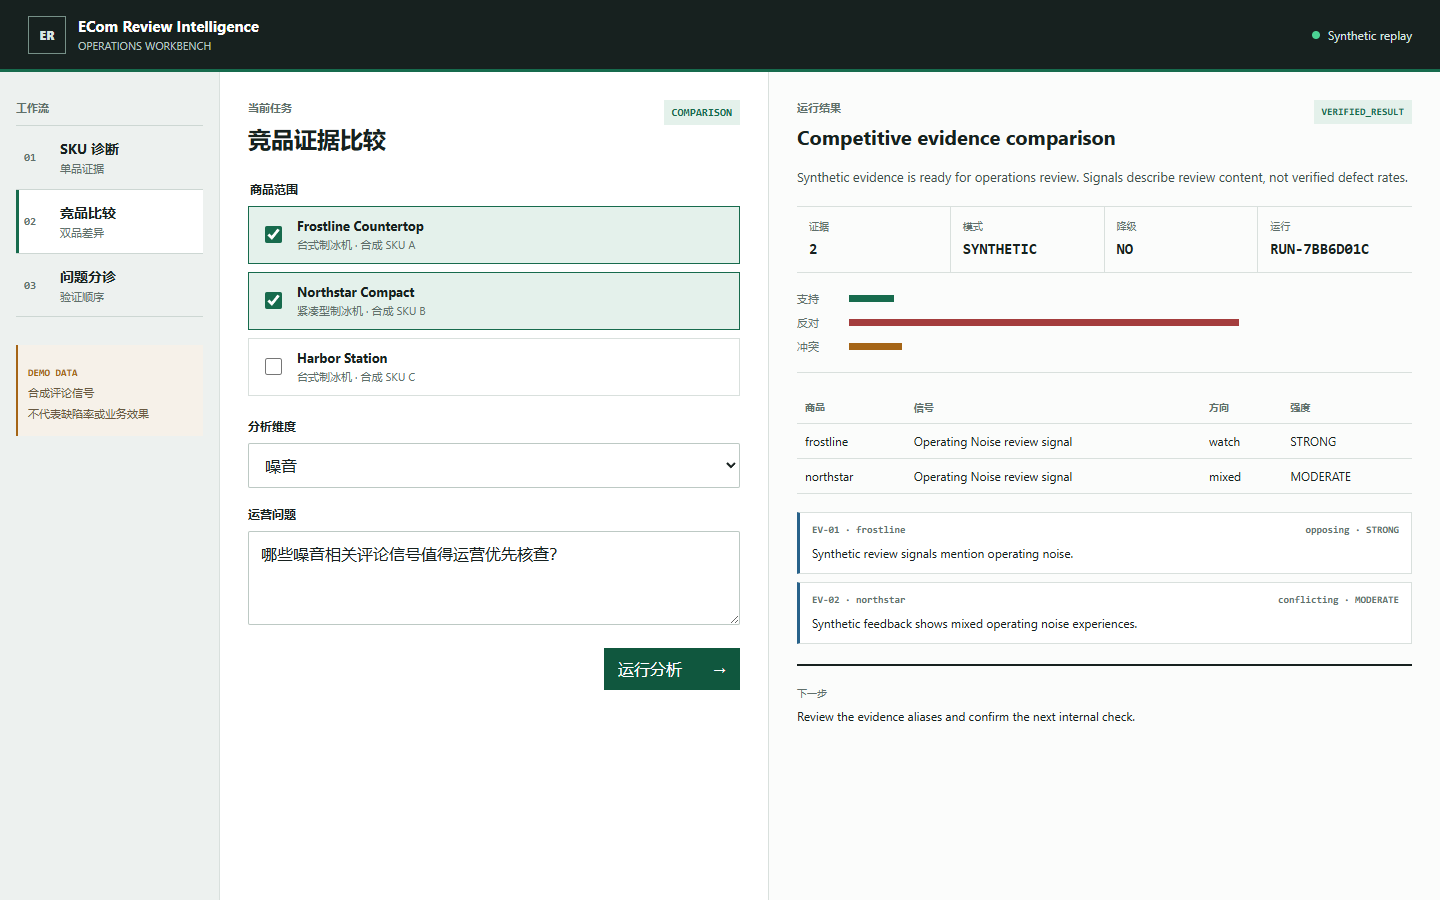
\includegraphics[width=\textwidth]{assets/p7-tour-03-comparison.png}%
  }{%
    \fbox{\parbox[c][45mm][c]{0.90\textwidth}{\centering
      此处放置电脑端截图\\
      \texttt{assets/p7-tour-03-comparison.png}\\
      比较结果、状态和证据区域}}
  }
  \caption{运行后查看状态、比较信号、证据卡和下一步。}
\end{figure}

此时，\textbf{左侧工作流导航}仍显示当前任务是竞品比较；\textbf{中间区域}保留原来的商品、维度和问题，便于回看“这份结果是在回答什么”；\textbf{运行按钮}已经触发一次受控运行，不应连续点击来制造多个不必要请求；\textbf{右侧状态}告诉你结果是否通过检查；\textbf{右侧证据}展示支持、反对或冲突的聚合信号和匿名证据卡，\textbf{下一步}给出需要运营人员继续核查的内部动作。\textbf{这一屏在项目中要展现什么：}系统输出的不只是文字，还要让人知道状态、证据数量和后续动作；它提供决策输入，不替运营人员宣布真实缺陷率。

\subsection*{比较页怎么读：先确认“同一把尺子”}

比较页最重要的不是哪一根横条更长，而是两个商品是否使用了同一个分析维度和同一类问题。截图中两个商品都放在“噪音”维度下，因此表格里的两行才有可比性。读图时依次检查：

\begin{enumerate}
  \item 中间是否真的勾选了两个商品；
  \item 下拉框中的分析维度是否相同；
  \item 右侧表格是否一行对应一个商品；
  \item 每一行能否回到自己的证据卡；
  \item 下一步是否仍然是“核查”，而不是直接宣布谁一定更好。
\end{enumerate}

这套读法的业务价值是减少“拿不同口径硬比较”的误判。例如，一个商品看噪音，另一个商品看制冰速度，即使最终文字很流畅，也不能支持采购或运营排序。比较工作流把商品范围、维度和输出行数固定下来，让运营人员知道差异来自哪里。

\begin{beginnerbox}
把比较结果先说成：“在同一个噪音维度下，两个候选商品出现了不同方向的评论信号，下一步分别回查证据。”不要说成：“A 的缺陷率比 B 高 20\%”或“A 一定应该下架”；当前截图没有这样的数据和授权。
\end{beginnerbox}

\begin{beginnerbox}
“支持、反对、冲突”是当前评论信号的方向；“证据数量”是本次允许使用的证据条数；它们都不是市场占比、缺陷率或销售损失。初次阅读时，把右侧理解成“证据提示板”即可。
\end{beginnerbox}

\section{遇到不确定时：系统先询问，而不是替你猜}

如果使用者没有指定唯一商品，只输入了一个可能对应多个商品的宽泛说法，系统会进入澄清状态。澄清不是报错，而是把必须由人决定的选择显式展示出来。

\begin{figure}[htbp]
  \centering
  \IfFileExists{assets/p7-tour-04-clarification.png}{%
    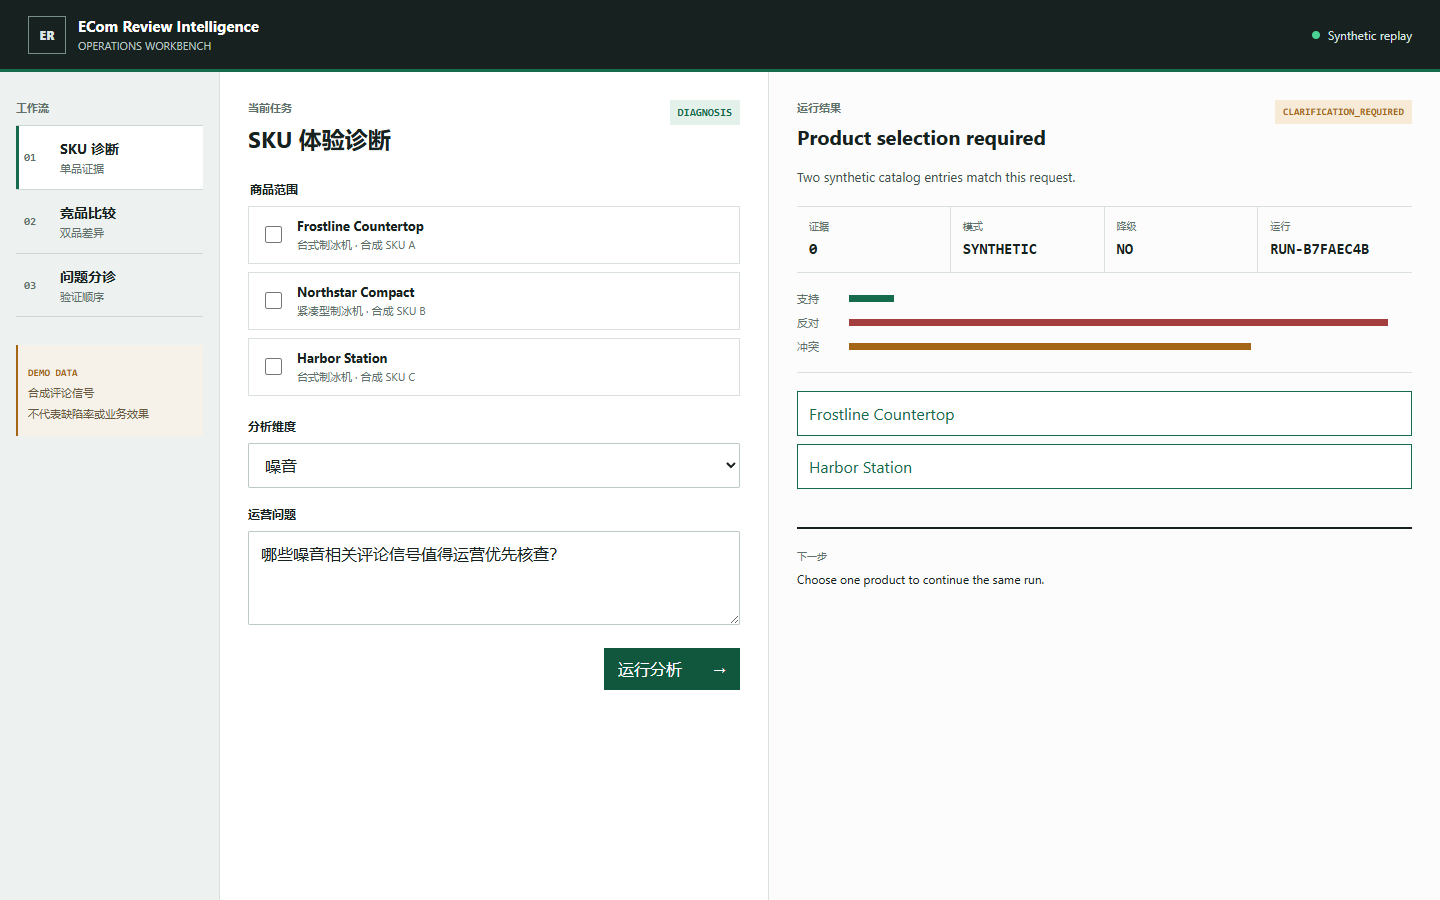
\includegraphics[width=\textwidth]{assets/p7-tour-04-clarification.png}%
  }{%
    \fbox{\parbox[c][45mm][c]{0.90\textwidth}{\centering
      此处放置电脑端截图\\
      \texttt{assets/p7-tour-04-clarification.png}\\
      需要选择候选商品的澄清页面}}
  }
  \caption{商品有多个候选时，进入澄清状态并选择授权候选。}
\end{figure}

这张图中，\textbf{左侧工作流导航}仍保留原任务类型；\textbf{中间商品与问题区域}显示原来填写的任务条件，并等待你从候选商品中作选择；\textbf{运行按钮}不会通过重复提交绕过选择；\textbf{右侧状态}明确显示需要澄清；\textbf{右侧证据与下一步}暂不假装有最终结论，而是告诉你先完成候选选择。\textbf{这一屏在项目中要展现什么：}当输入不够明确时，系统把决策交还给使用者，并保存这次任务以便继续。

澄清完成后，使用者点击一个已授权候选，系统恢复同一任务继续运行。这就是 checkpoint（暂停时保存的任务状态）最直观的含义：它像一张暂存的工作单，不需要从头猜一遍，也不允许选择候选列表之外的商品。

\subsection*{澄清页怎么读：这是安全功能，不是系统坏了}

澄清页右侧没有最终证据卡，是因为“到底分析哪个商品”这个前提还没有确定。它把模型不能安全替人决定的部分显式交还给使用者。对运营来说，这能避免把甲商品的评论误归到乙商品上；对工程来说，这能把一次运行停在明确状态，等人选择后再从原位置继续。

看到 \texttt{CLARIFICATION\_REQUIRED} 时，按三步处理：

\begin{enumerate}
  \item 看候选列表，确认每个候选的名称和上下文；
  \item 选择自己有权限确认的商品，不要凭相似名称猜测；
  \item 回到同一个运行，继续看状态、证据和下一步。
\end{enumerate}

这张图体现的价值是“宁可多问一次，也不把错误对象的证据交给业务”。它也是后面学习 checkpoint、恢复、审计和人工接管的最直观入口。

\section{从简单到完整：你正在逐渐学会哪些功能}

不要把工作台理解成一次性学会的“大模型聊天框”。可以按下面的能力梯度学习：

\begin{longtable}{>{\raggedright\arraybackslash}p{0.16\textwidth}>{\raggedright\arraybackslash}p{0.33\textwidth}>{\raggedright\arraybackslash}p{0.33\textwidth}}
\toprule
学习顺序 & 先学会什么 & 学会后的实际作用 \\
\midrule
\endfirsthead
\toprule
学习顺序 & 先学会什么 & 学会后的实际作用 \\
\midrule
\endhead
第 1 步 & 填写商品、维度和运营问题。 & 把模糊需求写成可执行任务。 \\
第 2 步 & 看状态、数量和证据卡。 & 判断结果是否有依据、是否需要人工复核。 \\
第 3 步 & 用同一维度比较多个商品。 & 给品类或运营团队提供可回查的差异线索。 \\
第 4 步 & 处理澄清和恢复。 & 遇到歧义时不猜错对象，并能继续原任务。 \\
第 5 步 & 理解工具、Verifier 和 Trace。 & 知道结果怎样被检索、检查和记录。 \\
第 6 步 & 连接真实 API 或真实用户试用。 & 在满足额外门槛后，评估延迟、成本和真实业务可用性。 \\
\bottomrule
\end{longtable}

前四步是“会用”；第五步是“能解释为什么相对可靠”；第六步才是“有资格讨论真实效果”。当前手册已经把前五步放进项目流程，但截图仍是 synthetic 演示，真实 API 和目标运营用户试用不应被截图替代。

\section{为什么页面有三种工作流}

三种工作流不是三个互相独立的 Agent，而是运营人员常见的三种问题形状。把它们分开，是为了让商品数量、输出形式和下一步动作都清楚。

\begin{longtable}{>{\raggedright\arraybackslash}p{0.22\textwidth}>{\raggedright\arraybackslash}p{0.32\textwidth}>{\raggedright\arraybackslash}p{0.32\textwidth}}
\toprule
页面任务 & 它回答什么 & 为什么不能混在一起 \\
\midrule
\endfirsthead
\toprule
页面任务 & 它回答什么 & 为什么不能混在一起 \\
\midrule
\endhead
单品体验诊断（diagnosis） & 一个商品在某个体验维度上有哪些支持、反对或冲突信号？ & 重点是看清一个商品的问题，不需要强行找出另一个商品。 \\
竞品证据比较（comparison） & 两个或多个商品在同一个维度上的证据有什么差异？ & 必须使用相同维度，否则比较的不是同一件事。 \\
问题分诊（triage） & 哪个运营问题值得先交给相应团队核查？ & 输出的是调查顺序，不等于缺陷严重度或财务损失排序。 \\
\bottomrule
\end{longtable}

如果把三种任务混成一个万能聊天框，模型可能既回答“这个商品怎么样”，又直接说“应该选哪个”，还把“先核查什么”说成“最严重的问题”。分开后，使用者能在运行前确认任务类型，程序也能为每种任务检查正确的商品数量和输出字段。

\section{把页面重新接回 P0--P7}

刚才的任务看起来只是勾选商品、选择维度和点击按钮，但页面背后依赖前面阶段已经做好的边界。可以按下面的顺序理解：

\begin{longtable}{>{\raggedright\arraybackslash}p{0.16\textwidth}>{\raggedright\arraybackslash}p{0.29\textwidth}>{\raggedright\arraybackslash}p{0.39\textwidth}}
\toprule
阶段 & 在刚才的任务中负责什么 & 初学者先这样理解 \\
\midrule
\endfirsthead
\toprule
阶段 & 在刚才的任务中负责什么 & 初学者先这样理解 \\
\midrule
\endhead
P0/P1 & 保证输入 & 先确认数据能用，再保证每次分析使用的是同一版输入。 \\
P2/P3 & 定义范围和维度 & 决定本项目看哪个类目，以及“噪音”这类问题怎样划分和标记。 \\
P4 & 提供证据 & 把允许使用的评论信号放进一个可以反复查询的本地证据账本。 \\
P5 & 比较检索 & 检查怎样更稳定地找到相关证据，比较方法是否真的引用了正确商品。 \\
P6 & 组织 Agent & 让模型按任务单规划，调用有限工具，并在出结果前接受复核。 \\
P7 & 提供工作台 & 把前面的能力放到电脑网页上，让运营人员可以填写任务、查看状态和继续澄清。 \\
\bottomrule
\end{longtable}

这也解释了为什么不能一开始就只写一个聊天框：如果 P0/P1 没有可靠输入，P2/P3 没有统一维度，P4 没有证据，P5 没有比较基线，P6 的 Agent 就算写出流畅答案，也不知道答案能不能被复核。P7 只是把已经有边界的能力呈现出来，并没有把演示页面变成业务效果证明。

\section{这一章学到什么，后面怎样读}

第一次使用时，你只需要掌握这条操作线：\textbf{选任务} $\rightarrow$ \textbf{选商品和维度} $\rightarrow$ \textbf{写运营问题} $\rightarrow$ \textbf{运行} $\rightarrow$ \textbf{看状态和证据} $\rightarrow$ \textbf{按下一步继续核查}。遇到多个商品命中时，先澄清再继续。

后面阅读 P0--P7 时，每一阶段都可以回到这个完整任务：这一阶段为页面中的哪一部分提供了保证？它解决了什么风险？如果拿掉它，右侧结果会失去什么可信度？这样学习路线就从“先学抽象 Agent”变成“先看一个业务任务，再逐步理解它为什么能够安全运行”。

\begin{interviewbox}
面试时可以这样介绍：“我先用一个竞品噪音反馈比较任务说明工作台的使用方式：运营选择两个商品和同一体验维度，运行后查看状态、聚合信号和可回查证据；输入有歧义时，系统先澄清并恢复原任务。这个页面是 P0--P6 的能力在 P7 的呈现，synthetic 截图只证明演示流程，不代表真人业务效果已经验证。”
\end{interviewbox}
